\chapter{Data management}

%Nos capítulos anteriores, mostrou-se como manipular superfícies, máscaras para segmentação
%e medições. É possível exibir ou ocultar e criar ou remover esses elementos pelo painel de
%gerenciamento de \textbf{Dados}, localizado no canto inferior esquerdo da tela do InVesalius.
%O painel é dividido em 3 abas: \textbf{Máscaras}, \textbf{Superfícies 3D} e \textbf{Medições},
%conforme mostra a figura \ref{fig:volumetric_data}. Cada uma das abas agrupa dados
%correspondentes aos elementos a que se referem.

Previously, it was shown how to manipulate surfaces, masks for segmentation and measurements. It is possible to show or
hide, and create or remove these elements at the \textbf{Data} management panel, located in the left inferior corner of
Invesalius. The panel is divided in 3 tabs: \textbf{Masks}, \textbf{3D Surfaces} and \textbf{Measurements}, shown in
figure \ref{fig:volumetric_data}. Each tab contains features corresponding to the elements it referes to.

%\begin{figure}[!htb]
%\centering
%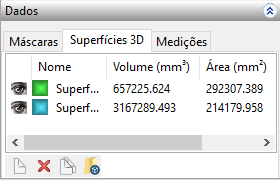
\includegraphics[scale=0.5]{medida_volumetrica}
%\caption{Gerenciamento de dados}
%\label{fig:volumetric_data}
%\end{figure}

\begin{figure}[!htb]
\centering
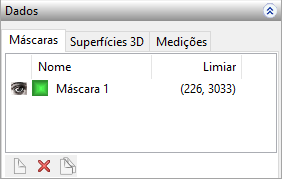
\includegraphics[scale=0.7]{painel_mask_manager_pt.png}
\caption{Data management}
\label{fig:volumetric_data}
\end{figure}

%Dentro de cada aba, aparece um painel dividido em linhas e colunas. Em cada linha, a primeira
%coluna determina a visualização do elemento listado naquela linha. Isto é, o ícone que
%representa um "olho" ativa ou desativa a exibição das máscaras, superfícies ou medições. Caso
%um desses elementos esteja em exibição, o ícone da figura \ref{fig:disable_mask} correspondente
%a ele também estará visível.

In each tab, there is a panel divided in rows and columns. First column of each line determines the visualization status
of the listed element. It means that the "eye" icon activates or deactivates the masks, surface or measurement exibition.
In case one of these elements is being exhibited, its corresponding icon shown in figure \ref{fig:disable_mask}, will
also be visible.

\newpage

\begin{figure}[!htb]
\centering
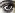
\includegraphics[scale=0.9]{eye}
\caption{Icon indicating the elements visibility}
\label{fig:disable_mask}
\end{figure}

%Algumas operações são possíveis sobre os dados. Por exemplo, para excluir um dado, é necessário
%primeiro selecionar seu nome, como mostra a figura \ref{fig:selected_mask} e, em seguida, clicar
%no atalho que a figura \ref{fig:delete_data} ilustra.

Some operations may be porformed with the data. For instance, to remove one element, it is necessary to first select
its name, show in figure \ref{fig:selected_mask} and next click in the shortcut illustrated in
figure \ref{fig:delete_data}.

\begin{figure}[!htb]
\centering
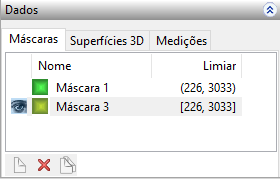
\includegraphics[scale=0.7]{painel_selected_mask_pt.png}
\caption{Data selected}
\label{fig:selected_mask}
\end{figure}


\begin{figure}[!htb]
\centering

\includegraphics[scale=0.8]{data_remove.png}
\caption{Remove data}
\label{fig:delete_data}
\end{figure}

%Para criar uma nova máscara, superfície ou medição, basta clicar no atalho ilustrado na figura
% \ref{fig:new_data}, desde que a respectiva aba esteja aberta.

To create a new mask, surface or measurement, click in the shortcut show in figure \ref{fig:new_data}, considering that
the corresponding tab must be open.

\begin{figure}[!htb]
\centering

\includegraphics[scale=0.8]{data_new.png}
\caption{New data}
\label{fig:new_data}
\end{figure}

%Para copiar um dado, basta selecioná-lo e clicar no atalho que a figura \ref{fig:duplicate_data}
%ilustra.

To duplicate a data, select it and click in the shortcut shown in figure \ref{fig:duplicate_data}.

\begin{figure}[!htb]
\centering

\includegraphics[scale=0.8]{data_duplicate.png}
\caption{Duplicate data}
\label{fig:duplicate_data}
\end{figure}


\newpage


\section{Masks}

%Na coluna \textbf{Nome}, são exibidos a cor e o nome atribuídos à máscara. Já a coluna
%\textbf{Limiar} exibe o intervalo de valores utilizado para criar a máscara. A figura
%\ref{fig:volumetric_data} mostra um exemplo.

At column \textbf{Name}, the mask's color and name are show. In turn, column \textbf{Threshold} show the value range
used to create the mask. Figure \ref{fig:volumetric_data} exhibits an example.

\section{3D Surface}

%Na coluna \textbf{Nome}, são exibidos a cor e o nome atribuídos à superfície. A coluna
%\textbf{Volume} mostra o volume total da superfície. Por fim, a coluna \textbf{Transparência}
%indica o nível de transparência em uso para exibir a superfície. A figura \ref{fig:surface_manager}
%traz um exemplo.

At column \textbf{Name}, the surface's color and name are show. Column \textbf{Volume} show the total surface volume.
Finally, column \textbf{Transparency} indicates the level of transparency in use for surface visualization.
Figure \ref{fig:surface_manager} shows an example.

\begin{figure}[!htb]
\centering
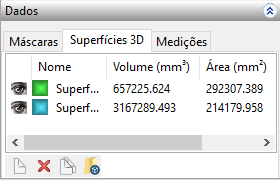
\includegraphics[scale=0.7]{painel_volumetric_measures_pt.png}
\caption{Surface manager}
\label{fig:surface_manager}
\end{figure}

\subsection{Import surface}

%É possível importar arquivos do tipo STL, OBJ, PLY e VTP (VTK Polydata File Format) com um projeto do InVesalius ativo,
%para isso é necessário clicar no ícone que é mostrado na figura~\ref{fig:import_stl},
%selecionar (figura~\ref{fig:import_surface}) o formato do arquivo que será importado e depois clicar no \textbf{Abrir}.

It is possible to import a file of type STL, OBJ, PLY or VTP (VTK Polydata File Format) with an active InVesalius
project. To do so, click in the icon shown in figure~\ref{fig:import_stl}, select the
format of the corresponding file, figure~\ref{fig:import_surface}, and click Open.

\begin{figure}[!htb]
\centering

\includegraphics[scale=0.8]{load_mesh.png}
\caption{Import Surface}
\label{fig:import_stl}
\end{figure}

\begin{figure}[!htb]
\centering
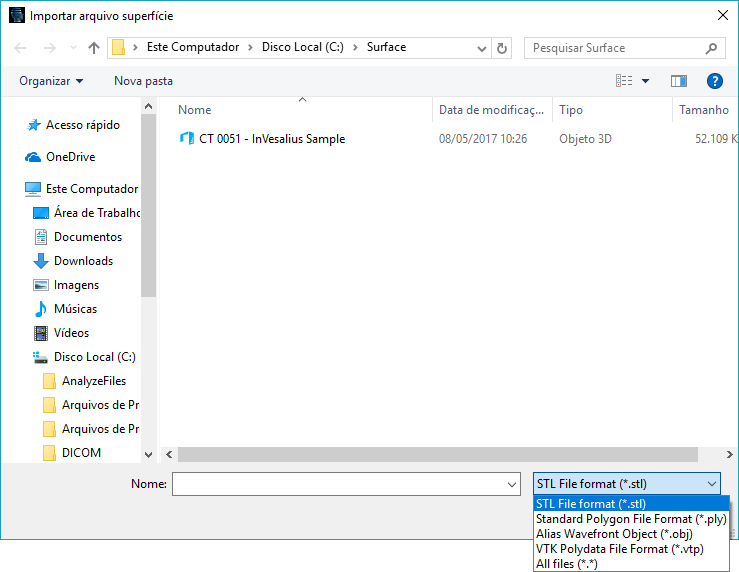
\includegraphics[scale=0.4]{import_surface_pt.png}
\caption{Window to import surface}
\label{fig:import_surface}
\end{figure}

\newpage


\section{Measurements}

%A aba \textbf{Medições} traz as seguintes informações. A coluna \textbf{Nome} exibe a cor e o
%nome atribuídos à medição. A coluna \textbf{Local} exibe onde a medição foi feita (imagem axial,
%coronal, sagital ou 3D), e \textbf{Tipo} indica o tipo da medida (linear ou angular). Por último,
% coluna \textbf{Valor} informa a medida propriamente dita. Veja a figura \ref{fig:manager_mensuares}.

The tab \textbf{Measurements} shows the following information. Column \textbf{Name} indicates the color and measurement
name. Column \textbf{Local} indicates where the measurement was taken (image axial, coronal, sagital or 3D), and
\textbf{Type} indicates the type of measurement (linear or angular). Finally, column \textbf{Value} shows the
measurement value. Figure \ref{fig:manager_mensuares} illustrates the \textbf{Measurements} tab.

\begin{figure}[!htb]
\centering
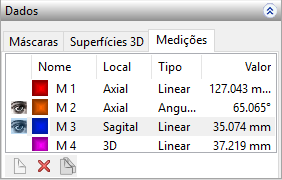
\includegraphics[scale=0.7]{painel_measures_manager_pt.png}
\caption{Data management}
\label{fig:manager_mensuares}
\end{figure}

